\chapter{High Data Complexity Power/EM 1} \label{cha:High Data Complexity Power/EM 1}

So far, we have attacked two cryptographic systems in the course:
\begin{itemize}
    \item \textbf{RSA:} using Montgomery reduction with time as a side-channel.
    \item \textbf{AES:} using simple power analysis
\end{itemize}

We attacked AES using simple power analysis.
We had a power trace as an input, consist of hundreds of thousands of points.
We created a classifier or dozen classifiers.
The classifier input is the power traces and the output is a list of the hamming weights of each byte of the state.

\textbf{Firstly, lets understand what hamming weights are.}
The Hamming weight of a string is the number of symbols that are different from the zero-symbol of the alphabet used. For example the hamming weight of 11101 is 4, as seen in the chart below. It is thus equivalent to the Hamming distance from the all-zero string of the same length.
The chart below is brought in order to show the hamming weight of different types of strings.

\begin{table}
    \caption{Hamming weights of different bit strings~\cite{hamming}}\label{hammingWeights}
    \begin{center}
    \begin{tabular}{ cc }
        \toprule
        String & Hamming Weight \\ 
        \midrule
        \textbf{111}0\textbf{1} & 4 \\ 
        \textbf{111}0\textbf{1}000 & 4 \\
        00000000 & 0 \\
        \textbf{789}0\textbf{1234}0\textbf{567} & 10 \\
        \bottomrule
    \end{tabular}
    \end{center}
\end{table}
The picture below is a nice visualization of how the hamming weight of binary numbers fluctuates when the binary number is growing.

\begin{figure}[!ht]
    \centering
    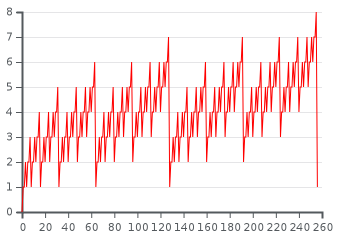
\includegraphics[width=0.8\textwidth]{images/Lecture6/HammingWeightBinary.png}
    \caption{Hamming weight for binary numbers (0-256)} \label{fig:HammingWeightBinary }
\end{figure}

For AES, we have 84 classifiers that we did not care about how these classifiers were created.
These classifiers can be created with every reasonable way to create a classifier.
We assume they take as input that power trace and output the hamming weight. 

A question arises: does the classifier look at the entire power trace?
Assume that the classifier wants to find the hamming weight of the first sub-bytes operation of AES.
In order to do this operation, we have to take the first byte of the plain text and the first byte of the key.
The sub-byte operation: look at the sub bytes table and replace the state with sub bytes of the state. 

Does the classifier need to look at the entire 1000 or 100,000 points of the trace?
Or maybe it needs to look at a certain limited amount of points in the trace?
The given power trace contains much redundant information.
The redundancy created because we started our measurement a while before the first sub-byte operation happens, these measurements are irrelevant for us.
The early measurement is just an arbitrary operation that happened before the encryption started.

\textbf{What is the requiered trace size} -
Assume we have an army of classifiers, each classifier is going to look at a certain number of points from the trace, ten, 15 or hundred points.
How to separate the points in the trace to the classifiers?
We will go into that a little bit during this chapter. 

We want to combine two attack methods: timing and simple power analysis, to take the best part of each one of these methods.
Combining them will improve the results.
This method is called differential power analysis.

In the timing attack, what is the threat model? 
What was the adversary allowed to do? 
The adversary allowed to send inputs to the device, 
get the outputs from the device, 
and measure how long it took.
The adversary was not necessary for controlling the inputs, 
he just had to know when the input was provided without knowing what the input value was.
He needed to know when was the input was when the output to find the time difference. 
The adversary had to measure many times and have many inputs, 
then he did some statistics to analyze it.
The various scenarios when we can justify a timing attack – when the device is available, or it is accessible across the web and so on.

What about simple power analysis? 
What was the threat model there? 
What did we allow to do with the device? 
First of all, we had to open the device, cut its power supply, and connect a power probe, the meter that measures the power consumption.
The attack is an invasive attack, and maybe it is considered less probable that we allowed doing that as attackers. 
If we are doing an electromagnetic probe, it would be less invasive, but we will still have to get very close to the device, but it would be less detectable. 

In the previous sections, we mentioned that to perform simple power analysis, we have an army of classifiers.
However, we did not mention how to train them and where their data came from.
Before we start the simple power analysis, we have an offline phase.
In this phase, we use a device which we can do reverse engineering and get really into it is internals. 
Maybe look at it with a microscope, or we can understand completely how it works, and then this device is similar to the DUT. 
The only thing we are not allowed to know as an adversary is the secret key.

What is the difference between the two devices? 
According to Kirchhoff's principles, the difference between our DUT to what we use to learn is the \textit{current}. 
  
How do we get this copy of the device in the real world?
Well, we can buy it, we can steal it, maybe buy it online. 
We have to have a very involve offline phase before we can do a simple power analysis.
We have to get close to the device that we want to attack and do reverse engineering.
If we justify it by buying stuff on eBay, we can go to the trash, and we can look at the datasheets.

The next phase in our attack is the \textit{online phase}. 
In simple power analysis, we can perform one or two simple measurements.
The problem with these measurements is that these measurements are our only chance to measure the device, and we have one trace that has to be very clean with very little noise. 
We cannot control this noise.
For example, if we take the measurements outside the lab, there will be some noise that we can not control. 
However, if we are using measurement equipment, the measurement equipment is going to add noise, and the DUT is introducing noise by itself.
Unfortunately, we cannot do so much about the noise in the simple power analysis scenario, because we only have the online phase.

\subsubsection{What can we do if we had a little noise and we don't have the exact key?}

\textit{That's exactly our problem with simple power analysis}

A problem that can arise from this noise is that we get one incorrect byte.
Can we find the right key by searching it around the guess?
Assume that we got AES key, which is 16 bytes long, and it is 8-bit implementation, and we tried the key and it is wrong.
Now, we try to check which byte is the wrong byte, by changing its value to every possible value.
How many attempts would we have to perform?
We start our search from the first byte, and we check all its possible values, if we did not find the right key, we are going to the second byte until we find the right key.
We have 256 options per position times and 16 bytes of the key.
That means that we have to perform 256*16 decryption operations.
However, how many decryption operations we have to do if we have more than one wrong bytes?
It is 16 choose 2 – to choose which 2 bytes to change, which is more or less 16 squared, so it is two to the power of $4\times2$.
We chose to byte, and then what we do is that we go over all the possible combinations of these bytes, which is two to the power of 16, so it is two to the power of $8+8=16$.
It grows up fast and it is going to be as bad as brute force pretty quickly.
We have to work very hard if we do not get the key right, it blows up exponentially.
The analysis here is by using byte and not bits because if we are looking at an 8-bit8-bit micro-controller, a lot of the operations will be byte-oriented, so it is going to be more likely to get the entire byte wrong.

\textbf{The solution to this problem is to have a more complex offline phase which prepare us for the online phase.}

Simple power-analysis will work fine if it is reasonable to conduct thousands of measurements on the same device in order to eliminate noise with statistics, however, it is not always practical.

\section{High Data Complexity Attacks}

(AKA: \textit{DPA} and \textit{CPA})

The main idea is to capture many traces and use statistics to recover the key.
The advantages of these methods are:
\begin{itemize}
    \item Does not require detailed information about DUT (save us the cost of doing reverse engineering to the device).
    \item Succeeds even under extreme noise.
\end{itemize}

On the other hand, the drawback is that the attack model is different now, we need to own the device. 
That may cause some people to think that this attack model is irrelevant because it is not practical. 
In truth, it might be practical in quite a wide range of situations.


\subsubsection{Why would we want someones secret?}

A good example of this is how TV suppliers calculate your bill.
You use your secret to identify yourself to the supplier. The suppliers can then decide which programs you are given access to, and how to charge you for accessing purchasable items (a movie, vod, etc \ldots). 
Consequently if someone were to obtain your secret somehow they would be able to watch anything at any cost. In the end you would be the one paying for it

\subsection{How complex power analysis works}

Until now, we knew about 2 ways of attacking with side channel:
\begin{enumerate}
    \item \textit{Timing Attack}
    \item \textit{Simple power analysis}
\end{enumerate}

When we used the timing attack, we tried many inputs, and the measurement for each input contained one output: for one input, we had the time it took. 
On the other hand, when we did Simple Power Analysis, for each input, we had a huge power trace (vector of points which indicates the power consumption over time for a given input). 
In other words, the data complexity was simple in both of these
methods - we had a $1d$ input. 
Now we will try to take it a step further, combine these methods, and create a new method with $2d$ input, which means now we have high data complexity. 
Instead of giving just the power trace, we will give as input the traces for various data at fixated points in time. 
We have a set of data ${D_1, D_2, ..., D_n}$ and we have the power trace of the system for each one of these inputs, at the time, i.e., the first point in the power trace for all these inputs, was taken at the same relative time. 
So now our output is not a vector but rather a Matrix $M_{DxT}$.

\begin{figure}[!ht]
    \centering
    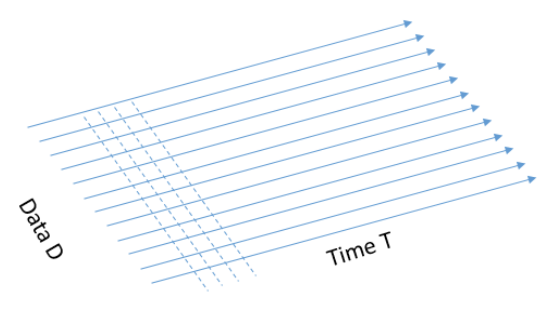
\includegraphics[width=0.8\textwidth]{images/Lecture6/DPA_Illustration.png}
    \caption{many measurements over time} \label{fig:DPA_Illustration}
\end{figure}

The suspicious reader should ask: how is it possible that we measure the power-traces of all the different data inputs all at the same time? 
That is indeed a challenge to align all the measurements along the time-line, and some of the countermeasures to the attack we present here will insert randomized operations or will change the clock speed so that we will have trouble aligning the power-traces along the time-line. 
If you are curious about that, you might find it interesting to look at the DPA book (the coursebook) and read about the countermeasures and how to overcome them.

\subsection{Using Vaizata method}
The next thing we are going to do is to use the Vaizata similarly to how we did it with timing attacks. 
When we did a timing attack, we guessed a bit of the key, and then we measured how much time it took. 
We are going to assume that sometimes the algorithm depends on the key; therefore, the power consumption will be depended on the key. 
Finally, we are going to check the measurements using some statistics tests. 

Unlike the timing attack where we knew that we measure the relevant data, when we used power analysis, we have a very long power trace where only a few points relevant to us and all the other points represent data that is not related to the key.

\textbf{Reminder:}

\begin{itemize}
\item Make a {simple assumption} about the implementation
\item Guess a {small part} of the key
\item Make an {hypothesis} about the effect of the guess on the execution
\item {Classify the measurements} according to the hypothesis
\item If we guessed right, the classification will be {statistically meaningful}
\end{itemize}

\begin{figure}[!ht]
    \centering
    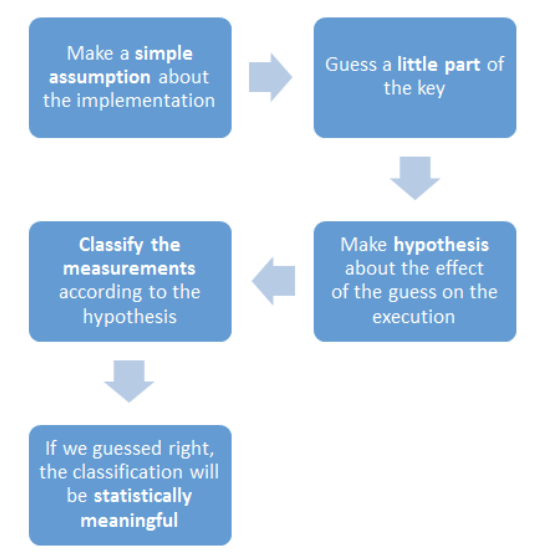
\includegraphics[height=0.9\textwidth]{images/Lecture6/vaizata.png}
    \caption{Vaizata method stages} \label{fig:vaizata}
\end{figure}

Now, we are looking for a stage during the AES algorithm, where a small number of bits of the key, affect a large amount of the bits in the state. 
The intuition here is that we want to find a stage in the algorithm, where the power consumption depends on the key value.

\begin{figure}[!ht]
    \centering
    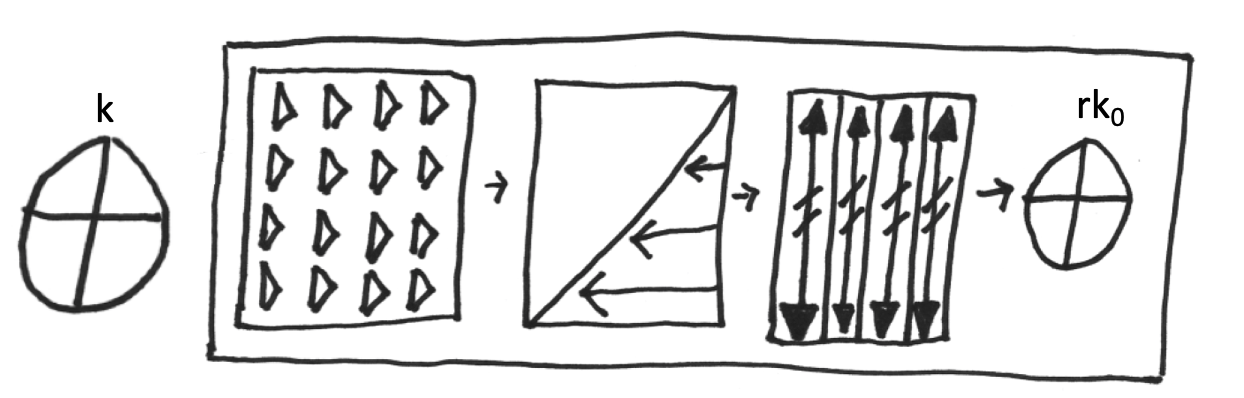
\includegraphics[width=0.8\textwidth]{images/Lecture6/AES-stages-figure.png}
    \caption{AES stages} \label{fig:aes-stages}
\end{figure}

We might consider measuring the power consumption just before the start of the algorithm, but in this case, the key does not affect the state.
Next, we have the add round key. 
After this operation, each bit of the key affects precisely one bit of the state.
Why is that? 
Because we essentially ``XOR" the key with the state, which so the first bit of the key affects the first bit of the state.

Our second operation will be \texttt{subbytes}. 
The \texttt{subbytes} operation is a value-based substitution, where each possible state value is mapped to a different value as defined by the substitution matrix. 
In this stage, every bit of the key affects 8 bits of the state! Why is that? 
If only one bit in the key were different, our add-around key would cause another bit of the state to change, and that would lead the \texttt{subbytes} look-up to bring an entirely different byte to the resulting state.

Next, we have \texttt{shiftRows}, where still every bit of the key affects 8 bits of the state. 
Why is that? 
Because we just moved the data, we did not diffused it.

And now we have the \texttt{MixColumns} operation. 
How many bits of the state now is affected by every bit of the key? 
In the \texttt{MixColumns} operation, each byte depends upon 4 bytes, and each byte is 8 bits that depend on the key. 
So we now have 32 bits of the state, which depends upon a single bit of the key.

As an attackers, we are going to focus on the point immediately after the \texttt{subbytes} and right before the \texttt{shiftRows}. 

So based on this information, what should be our Vaizata assumption?
The assumption is that is the power consumption of the device is the function of the data, so if we change the data, the power consumption changes.
(A counter-measure for that will be to build a machine that consumes the maximum power all the time).

Similarly to our attack on the RSA algorithm, where we guessed a bit of the key, we are going now to guess a byte of the key (since AES is byte-oriented). 
When we attacked RSA, we have split our data into two groups and then conducted $t-test$, but since we guess a byte, now we have 256 groups.

We know the value of the plaintext (it is given), and we are making a guess about the key, but how will we know the value of the \texttt{subbytes}? 
By Kerckhoffs's principle, which means that everything regarding the algorithm but the key is shared publicly.

So for each data point, and each byte guesses, we have 256 options. 
255 out of them will be meaningless, and only one is the correct guess, which should have statistical significance.

\begin{figure}[!ht]
    \centering
    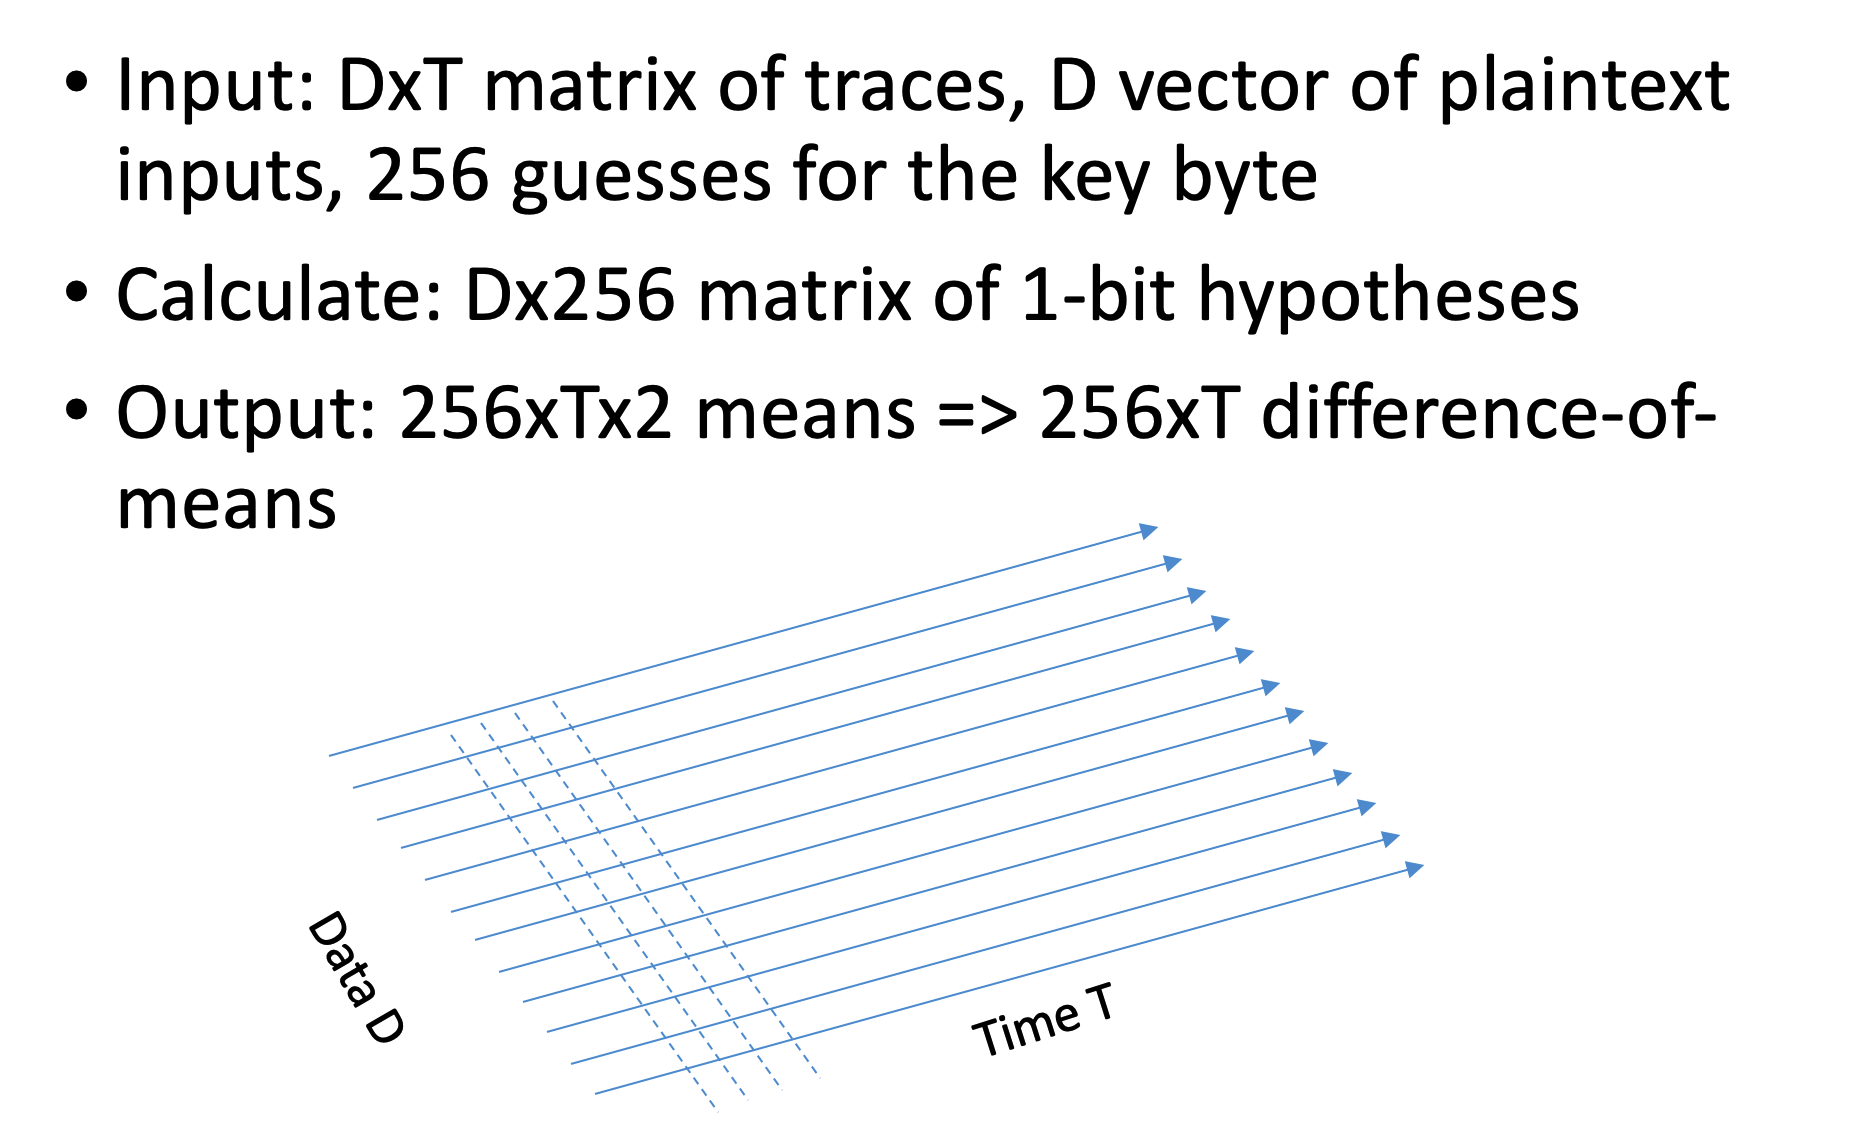
\includegraphics[width=0.8\textwidth]{images/Lecture6/dpa-separation-figure.png}
    \caption{The way we separate the data to groups based on the guess} \label{fig:dpa-separation-figure}
\end{figure}


The problem is that we have many different points each time, and we shall see a difference only at a certain point. 
Therefore our actions are as follows: for each guess, we split the measurements into two sets, and we measure the difference between the means of their power traces on every point of time. 
At most of the points, the difference will not be significant, except to the point where the guess was made correctly. 
We illustrate it at \Cref{fig:meansDiffFigure}.

\begin{figure}[!ht]
    \centering
    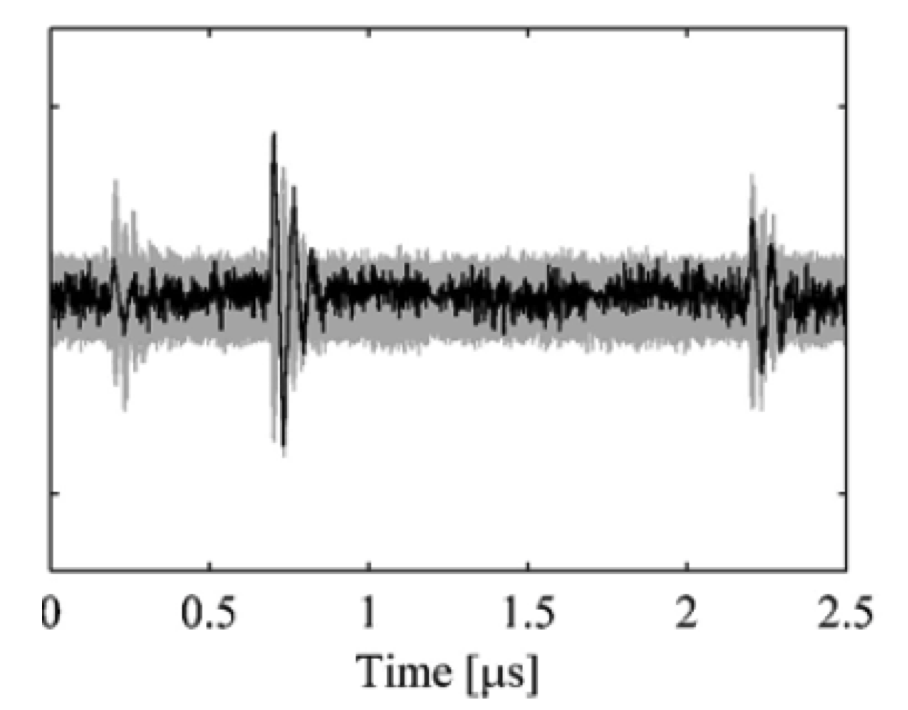
\includegraphics[width=0.8\textwidth]{images/Lecture6/meansDiffFigure.png}
    \caption{the difference of means as a function of time}
    \label{fig:meansDiffFigure}
\end{figure}

On the $X-axis$ we have the time, and on the $Y-axis$, there is the difference of means. 
In Gray, we can see the noise, and even if we guessed the correct key, we have a lot of similar points, because not all the times depend on the key. 
But we can see in the figure the moments of the peaks in the means
differences, these moments are also called ``the right times".
These essentially should be the moments of the sub-bytes. 
If we incorrectly picked a peak, which is a ghost noise, like in a point when we xor the plain the with the key, then we will not be able to find meaningful separation later on.

\section{DPA Lab}
In the class example, we attacked AES algorithm with 200 traces with size $30,000$ using an example data from the \textit{Power Analysis Attacks} book, and we visualized the process. 
First, we load the data and plot it in \Cref{fig:traceByTime} with the following axes: $X-Axis$ will be the time and $Y-Axis$ will be the trace number.
In addition, we had a dimension of color intensity, which will depend on the power consumption.

\begin{figure}[!ht]
    \centering
    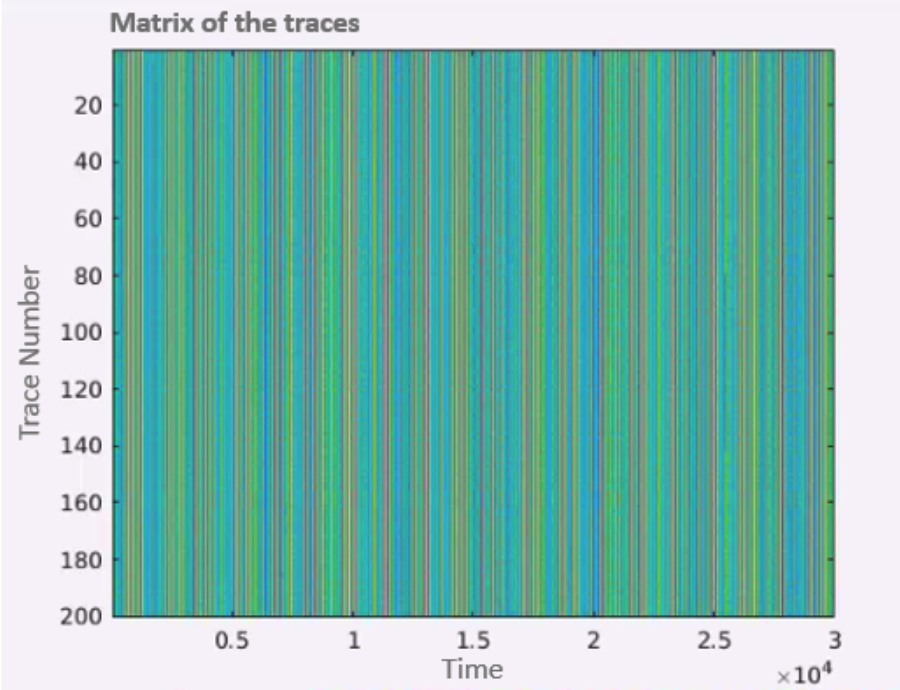
\includegraphics[width=0.8\textwidth]{images/Lecture6/traceByTime.png}
    \caption{the traces' power consumption by time} \label{fig:traceByTime}
\end{figure}

In plot \ref{fig:traceByTime}, there are very aligned columns which indicate that the traces are appropriately aligned. 
Our goal is to separate the power traces of the correct key from all the other traces. 
To do that, we start by showing in \Cref{fig:2traces-by-time} by comparing the power consumption of two traces based on time.

\begin{figure}[!ht]
    \centering
    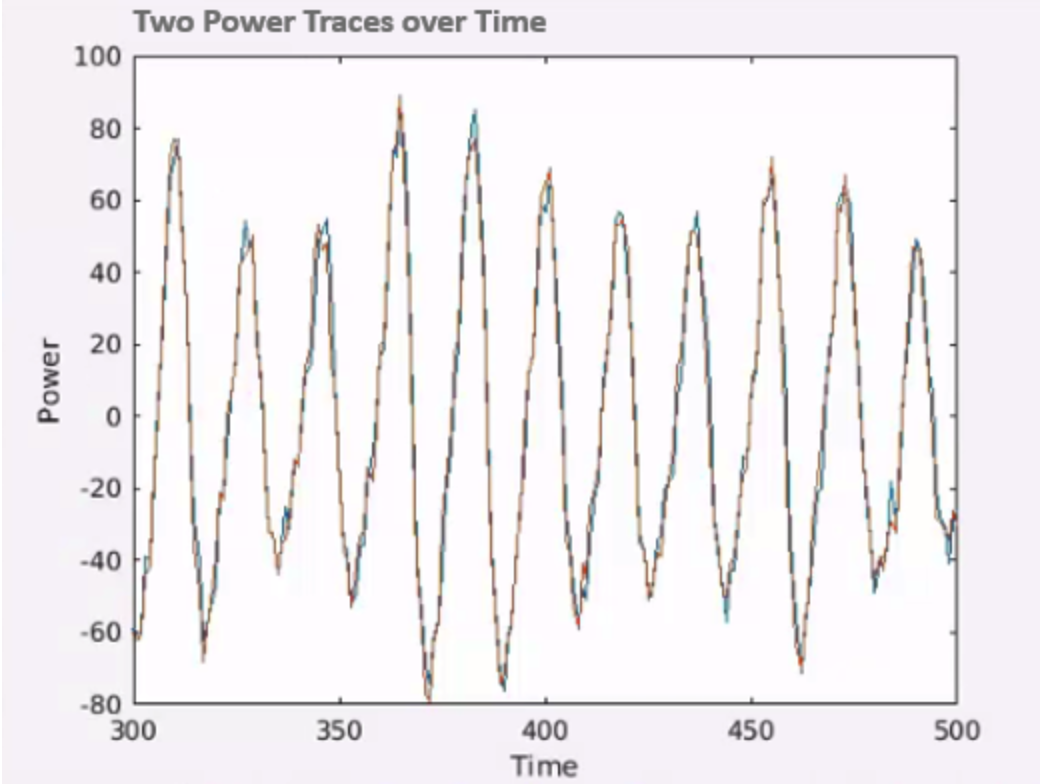
\includegraphics[width=0.8\textwidth]{images/Lecture6/2traces-by-time.png}
    \caption{2 groups of traces by times} \label{fig:2traces-by-time}
\end{figure}

We can see that both of them overlap, but if we had a difference, we would be able to find a separation on this graph.
Therefore, in \Cref{fig:intensity_by_guess}, we test for each key guess and input, what was the power consumption, whereas yellow represents less power and blue more power.

\begin{figure}[!ht]
    \centering
    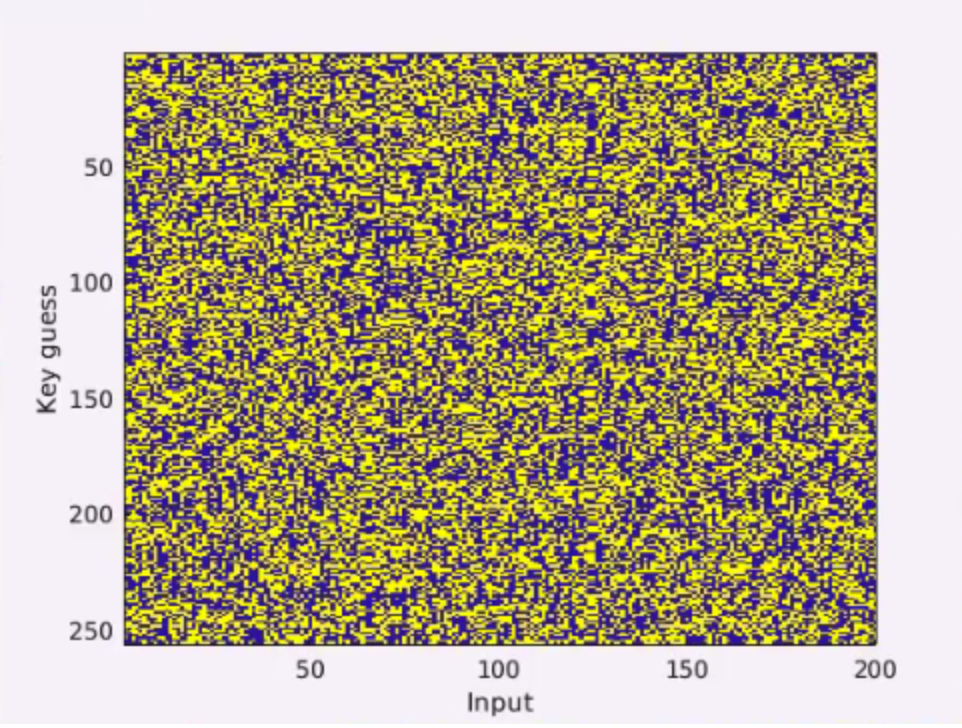
\includegraphics[width=0.8\textwidth]{images/Lecture6/intensity_by_guess.png}
    \caption{power consumption by guess and input} \label{fig:intensity_by_guess}
\end{figure}

Now we calculate the mean of power consumption for each guess, and we plot if over time.

\begin{figure}[!ht]
    \centering
    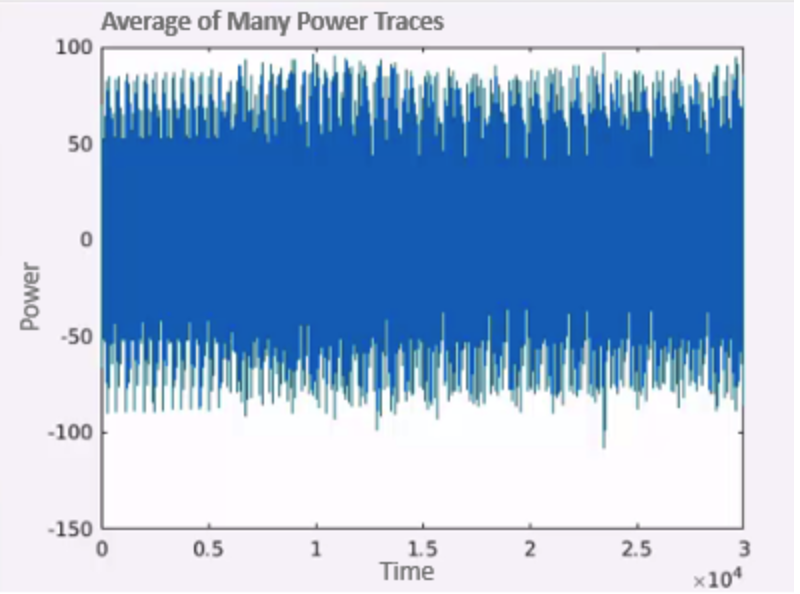
\includegraphics[width=0.8\textwidth]{images/Lecture6/avg_of_many_traces.png}
    \caption{mean of each guess across the different inputs by time} \label{fig:avg_of_many_traces}
\end{figure}


If we did the split correctly, this power trace average would be different from all the other 255 graphs. 
The problem with this chart is that we need to check many graphs, so we need something that shows the distance of means for all the guesses. 
A better graph will be to plot the distance of means of each key guess by time and then to search for the moment with the maximum difference (``the right time") like in \Cref{fig:intensity_represents_means_diff}.

\begin{figure}[!ht]
    \centering
    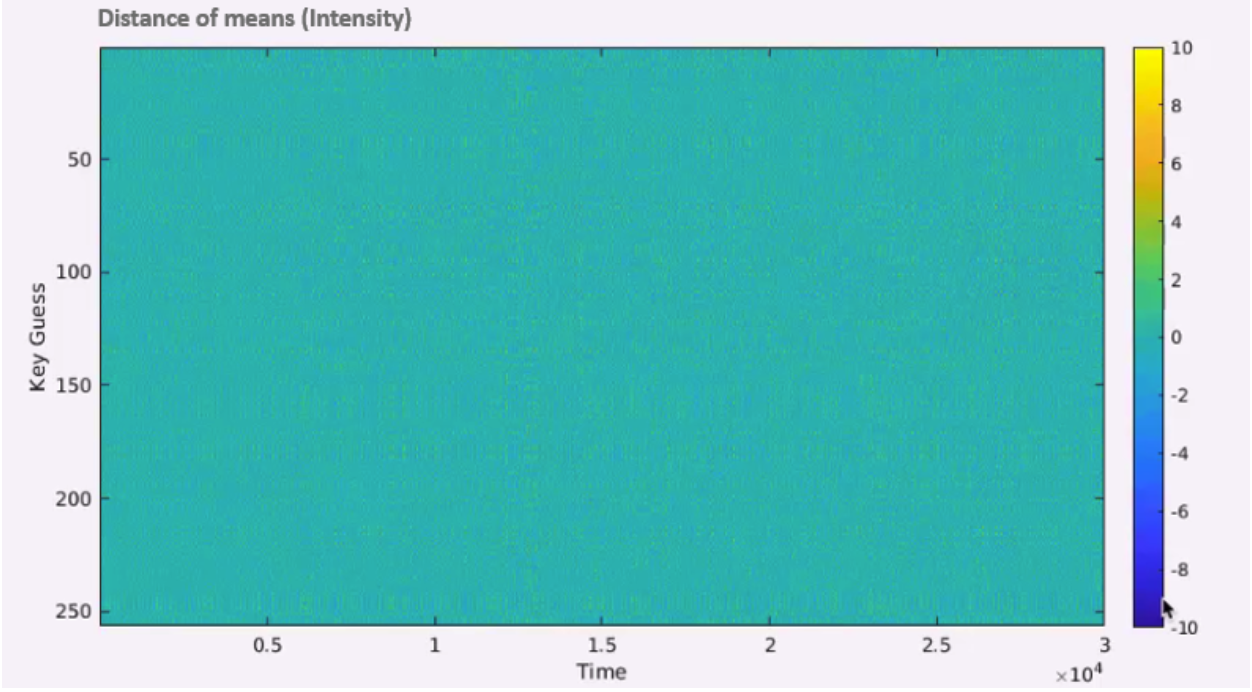
\includegraphics[width=0.8\textwidth]{images/Lecture6/intensity_represents_means_diff.png}
    \caption{distance of means by time and key guess, color intensity represents the distance} \label{fig:intensity_represents_means_diff}
\end{figure}

While it might be hard to spot it on this chart, there is a certain point of time where the difference is $8.91$, and at all the other points, it is somewhere near zero, as we can see on the charts.

What if we focus on the correct time across the different key guesses? We should be able to spot the correct guess, as shown in \Cref{fig:the-correct-time}.

\begin{figure}[!ht]
    \centering
    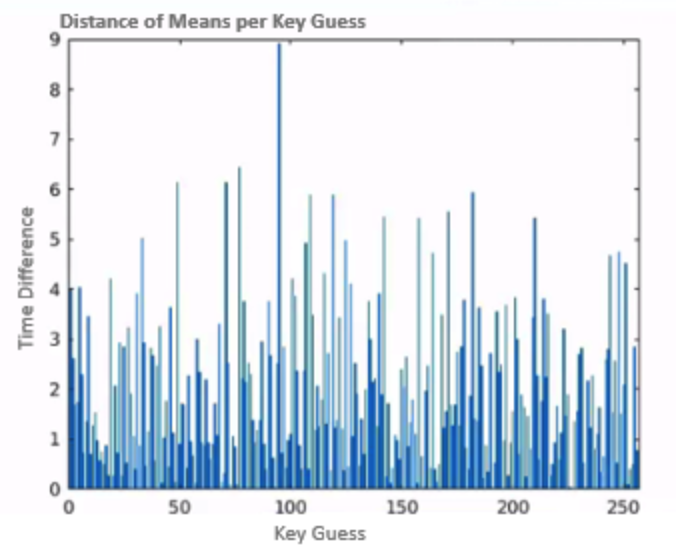
\includegraphics[width=0.8\textwidth]{images/Lecture6/the-correct-time.png}
    \caption{means distance at the correct time} \label{fig:the-correct-time}
\end{figure}

We finish by plotting the distance of means across time for all the keys, we can see in green the distance of means for the correct key, and we can see that at the right time, it is separated from the other keys as shown in \Cref{fig:all}.

\begin{figure}[!ht]
    \centering
    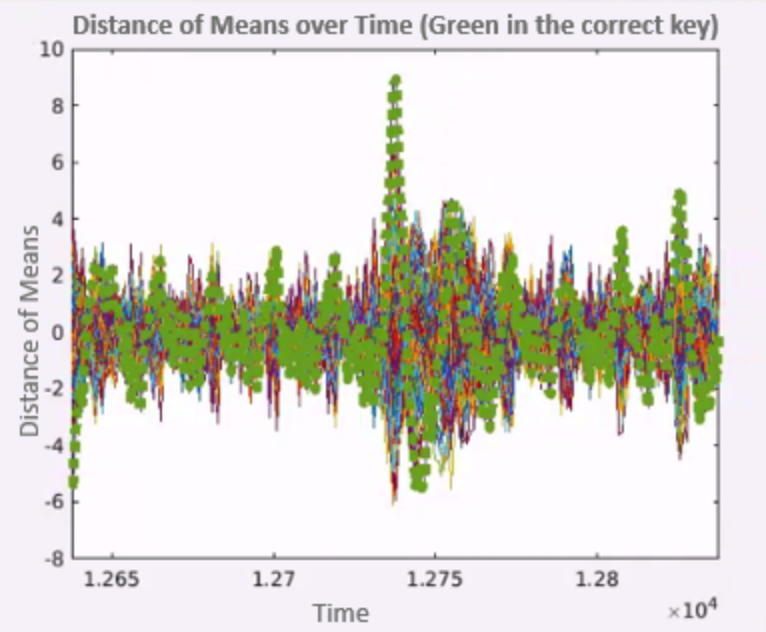
\includegraphics[width=0.8\textwidth]{images/Lecture6/all.png}
    \caption{distance of means for all key guesses across time \linebreak[4]} \label{fig:all}
\end{figure}

\subsubsection{Research Highlights}

    \begin{itemize}
        \item   This paper \cite{kocher1999differential} by Paul Kocher examines specific methods for analyzing power consumption measurements to find secret keys from tamper resistant devices.

        The paper presents the Differential Power Analysis subject comprehensively, its background, Simple power analysis, demonstration of DES algorithm attack, attacks on additional encryption algorithms using DPA and counter measures for DPA.
        It’s also discussed approaches for building cryptosystems that can operate securely in existing hardware that leaks information.
        \item Another article publish on 2005 \cite{mangard2005successfully} presents an attack on masked AES Hardware implementations.
        During the last years, several masking schemes for AES have
        been proposed to secure hardware implementations against DPA attacks.
        In order to investigate the effectiveness of these countermeasures in practice,
        the researchers responsible for the article designed and manufactured an ASIC. The chip features an
        unmasked and two masked AES-128 encryption engines that can be attacked
        independently.
        In addition to conventional DPA attacks on the output of registers,
        they have also mounted attacks on the output of logic gates. Based on
        simulations and physical measurements they show that the unmasked and
        masked implementations leak side-channel information due to glitches
        at the output of logic gates. It turns out that masking the AES S-Boxes does not prevent DPA attacks, if glitches occur in the circuit. However, an attacker usually does not have easy access to the back-annotated
        netlist of a product.
        \item This Article posted by Stefan Mangard \cite{mangard2004hardware}
        maintain that  Many hardware countermeasures against differential power analysis (DPA) attacks have been developed during the last years. Designers of cryptographic devices using such countermeasures to protect their devices have the challenging task to select and implement a suitable combination of countermeasures. Every device has different requirements, and so there is no universal solution to protect devices against DPA  attacks.

        In this article, a statistical approach is pursued to determine the effect of hardware countermeasures on the number of samples needed in DPA attacks. This approach results in a calculation method that enables designers to assess the resistance of their devices against DPA attacks throughout the design process. This way, different combinations of countermeasures can be easily compared and costly design iterations can be avoided.
        \item This article \cite{herbst2006aes} presents a countermeasure to Power Analysis attack on AES.
        The article describes an efficient AES software implementation that is well suited for 8-bit smart cards and resistant against power analysis attacks. Our implementation masks the intermediate results and randomizes the sequence of operations at the beginning and the end of the AES execution. Because of the masking, it is secure against simple power analysis attacks, template attacks and first-order DPA attacks. 
        Due to the combination of masking and randomization, it is resistant against higher-order DPA attacks. Resistant means that many measurements is required for a successful attack. 

        The implementation shown in the article compares well with other protected and unprotected AES software implementations for smart cards. The practical attacks that we have performed support our theoretical estimates about the security of the countermeasures.
        This article also includes a practical evaluation of the countermeasures. The results prove the theoretical assessment of the countermeasures to be correct.
    \end{itemize}
